
\documentclass[tikz,border=0pt]{standalone}
\usepackage{amsmath}
% Preamble (make sure you have these)
\usepackage{tikz}
\usepackage{xcolor}
\usepackage{amssymb}
\usetikzlibrary{decorations.pathreplacing}
\usepackage{pgfplots}
\usepackage{braket}
\pgfplotsset{compat=1.18}
\usetikzlibrary{positioning,calc,arrows.meta}
\usetikzlibrary{arrows.meta,positioning,calc}

\begin{document}
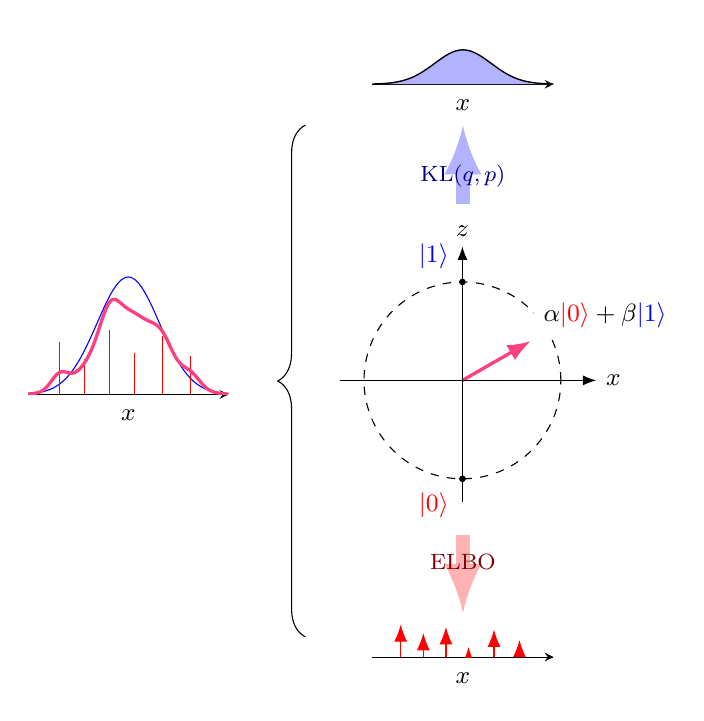
\begin{tikzpicture}[
    >=Latex,
    font=\small,
    col/.style={minimum width=0.30\textwidth},
  ]
  
  % ---------- Parameters ----------
  \def\xmin{-3.2}
  \def\xmax{3.2}
  \def\ymin{0}
  \def\ymax{0.55}
  
  % ---------- Left column: two axis plots ----------
  \node[col] (L) {};
  
  \node[anchor=north] (Ltop) at ([xshift=0\textwidth,yshift=0.35\textwidth]0,0) {};
  \begin{axis}[
    at={(Ltop)}, anchor=north,
    width=0.32\textwidth, height=0.18\textwidth,
    xmin=\xmin, xmax=\xmax, ymin=\ymin, ymax=\ymax,
    axis x line=bottom,
    axis y line=none,
    xtick=\empty, ytick=\empty,
    xlabel={$x$}, ylabel={$p(x)$},
    % title={\color{blue}$\ket{1}$: Gaussian},
    title style={font=\small},
  ]
    % Standard normal pdf (scaled a bit for nice view)
    \addplot[domain=\xmin:\xmax, samples=200, line width=0.5pt,fill=blue!30] {0.399*exp(-x^2/2)};
  \end{axis}
  
  \node[anchor=north] (Lbot) at ([xshift=0\textwidth,yshift=-0.25\textwidth]0,0) {};
  \begin{axis}[
    at={(Lbot)}, anchor=north,
    width=0.32\textwidth, height=0.18\textwidth,
    xmin=\xmin, xmax=\xmax, ymin=\ymin, ymax=\ymax,
    axis x line=bottom,
axis y line=none,
    xtick=\empty, ytick=\empty,
    xlabel={$x$}, ylabel={$p(x)$},
    % title={\color{red}$\ket{0}$: Discrete},
    title style={font=\small},
  ]
    % "Multi-delta" as spikes (stems)
    % --- inside the axis ---
\def\ybase{0.00} % baseline（你想要的基线高度）

% 可选：先画 baseline
\addplot[domain=\xmin:\xmax, samples=2, line width=0.3pt] {\ybase};

% 逐个画从 baseline 指向 y 的箭头
\pgfplotsextra{
  \foreach \xx/\yy in {
    -2.2/0.38,
    -1.4/0.28,
    -0.6/0.35,
     0.2/0.12,
     1.1/0.32,
     2.0/0.20
  }{
    \draw[-{Latex[length=2.2mm]}, line width=0.5pt,red]
      (axis cs:\xx,\ybase) -- (axis cs:\xx,\yy);
  }
}

  \end{axis}
 \begin{scope}[shift={(0.6,0)}]
  % ---------- Middle column: Bloch-sphere-like diagram ----------
  \node[col] (M) at ([xshift=0.02\textwidth]0,0) {};
  
  % Sphere center
  \coordinate (C) at ([xshift=-0.05\textwidth,yshift=-0.02\textwidth]0,0);
  
  % Draw sphere (as circle + a couple of ellipses)
  \draw[dashed] (C) circle[radius=1.25cm];
%   \draw[thick] (C) ellipse[x radius=1.25cm, y radius=0.45cm];      % equator
%   \draw[thick, dashed] ($(C)+(0,0)$) ellipse[x radius=0.55cm, y radius=1.25cm]; % meridian-ish
\begin{scope}[shift={(-0.6,0)}]
\draw[line width=5pt,-latex,blue!30]
  (0,2) -- (0,3)
  node[pos=0.35, rotate=0, blue!50!black] {\footnotesize KL$(q,p)$};

\draw[line width=5pt,-latex,red!30]
  (0,-2.2) -- (0,-3.2)
  node[pos=0.35, rotate=0, red!50!black] {\footnotesize ELBO};
\end{scope}
\draw[decorate,decoration={brace,amplitude=10pt}]
  (-2.6,-3.5) -- (-2.6,3);
  % Poles
  \coordinate (N) at ($(C)+(0,1.25cm)$);
  \coordinate (S) at ($(C)+(0,-1.25cm)$);
  
  \fill (N) circle[radius=1.2pt];
  \fill (S) circle[radius=1.2pt];
  
  \node[below left=2pt,red] at (S) {$\ket{0}$};
  \node[above left=2pt,blue] at (N) {$\ket{1}$};
  
  % A "state vector" showing mixture direction
  \draw[->, very thick,orange!50!magenta] (C) -- ($(C)+(0.87cm,0.5cm)$) node[black,fill=white,midway, above right=8pt and 13pt] {$\alpha{\color{red}\ket{0}}+\beta{\color{blue}\ket{1}}$};
  
  % Small axis arrows for aesthetics
  \draw[->] ($(C)+(-1.55cm,0)$) -- ($(C)+(1.70cm,0)$) node[right] {$x$};
  \draw[->] ($(C)+(0,-1.55cm)$) -- ($(C)+(0,1.70cm)$) node[above] {$z$};
  
%   \node[align=center] at ($(C)+(0,-2.05cm)$) {Latent ``state''\\(mixture intuition)};
  
  % ---------- Right column: mixture distribution ----------
%   \node[col] (R) at ([xshift=0.38\textwidth]0,0) {};
  
  \node[anchor=center] (Rax) at ([xshift=-0.4\textwidth,yshift=0.05\textwidth]0,0) {};
 \end{scope}
  \begin{axis}[
    at={(Rax)}, anchor=center,
    width=0.34\textwidth, height=0.30\textwidth,
    xmin=\xmin, xmax=\xmax, ymin=\ymin, ymax=\ymax,
    axis x line=bottom,
    axis y line=none,
    xtick=\empty,   % 或 xtick=\empty 如果你连刻度也不要
    ytick=\empty,
    xlabel={$x$}, ylabel={},
    title={},
    legend style={draw=none},
    legend entries={},
  ]
    % Gaussian component
    \addplot[domain=\xmin:\xmax, samples=200,blue] {0.399*exp(-x^2/2)};
    % \addlegendentry{Gaussian}
    % Delta-spikes component (scaled)
    \addplot[ycomb,red] coordinates {
      (-2.2,0.18) (-1.4,0.12) (-0.6,0.22) (0.2,0.14) (1.1,0.20) (2.0,0.13)
    };
    % \addlegendentry{multi-$\delta$}
  
    % A simple "mixture" curve: Gaussian + a few bumps (just for illustration)
    \addplot[domain=\xmin:\xmax, samples=200,very thick,orange!50!magenta] {0.70*(0.399*exp(-x^2/2))
      +0.08*exp(-(x+0.6)^2/0.18)
      +0.06*exp(-(x-1.1)^2/0.22)
      +0.05*exp(-(x+2.2)^2/0.15)
      +0.04*exp(-(x-2.0)^2/0.18)};
    % \addlegendentry{mixture (illustrative)}
  \end{axis}
  
  % ---------- Column labels (optional) ----------
%   \node[font=\small\bfseries] at ([xshift=-0.36\textwidth,yshift=0.15\textwidth]0,0) {Left: 1D views};
%   \node[font=\small\bfseries] at ([xshift=0.00\textwidth,yshift=0.15\textwidth]0,0) {Middle: latent picture};
%   \node[font=\small\bfseries] at ([xshift=0.36\textwidth,yshift=0.15\textwidth]0,0) {Right: blended};
  
  \end{tikzpicture}
\end{document}